\documentclass[letter, 12pt]{article}
\usepackage[utf8]{inputenc}
\usepackage[T1]{fontenc}
\usepackage[spanish]{babel}
\usepackage{graphicx}
\usepackage{tabularx} % Para ajuste automático de tablas
\usepackage{booktabs} % Mejora el diseño de la tabla
\usepackage{subcaption}
\usepackage{amsmath}
\usepackage{geometry}
\usepackage{titling}
\usepackage[colorlinks=true, linkcolor=blue, citecolor=blue, urlcolor=blue]{hyperref}

\usepackage{authblk}
\geometry{left=2cm, right=2cm, top=2cm, bottom=2cm}

\usepackage{tikz}
\usetikzlibrary{shapes.geometric, arrows.meta, positioning, calc}

\definecolor{startcolor}{RGB}{230, 240, 250}
\definecolor{processcolor}{RGB}{250, 250, 250}
\definecolor{decisioncolor}{RGB}{255, 245, 230}
\definecolor{linecolor}{RGB}{50, 50, 50}

\tikzstyle{startstop} = [draw=linecolor, rectangle, rounded corners=12pt, minimum width=2.5cm, minimum height=0.8cm, text centered, fill=startcolor, font=\scriptsize\bfseries, line width=0.8pt]
\tikzstyle{process} = [draw=linecolor, rectangle, minimum width=6cm, minimum height=1cm, text centered, text width=6.5cm, fill=processcolor, font=\scriptsize, line width=0.8pt]
\tikzstyle{decision} = [draw=linecolor, diamond, aspect=2, minimum width=3.5cm, minimum height=1.2cm, text centered, text width=3.5cm, fill=decisioncolor, font=\scriptsize, line width=0.8pt]
\tikzstyle{arrow} = [thick,->,>=Stealth,color=linecolor]

% Configuración de la portada
\title{
    \textbf{Desarrollo e implementación de redes neuronales de impulso usando celdas estandar neuromórficas} \\ \vspace{1cm} \Large Plan de trabajo - SEES
\author{\Large Jorge Alejandro Juárez Lora \\ CINVESTAV \\ CDMX}
}

\begin{document}

% Portada en página separada
\begin{titlepage}
    \centering
    \vspace{4cm}
    {\Huge \textbf{Desarrollo e implementación de redes neuronales de impulso usando celdas estandar neuromórficas} \par}
    \vspace{1.5cm}
    \vspace{2cm}
    {\Large Autor: Dr Jorge Alejandro Juárez Lora \par}
    \vspace{0.5cm}
         {\Large CINVESTAV - SEES - CDMX \par}
    % \vspace{0.5cm}
    % {\Large UNAM \par}
    \vspace{3cm}
    {\Large Julio 2026 \par}
    \vfill
\end{titlepage}

% Índice
\tableofcontents
\newpage

\section{Introducción}
\subsection{Planteamiento del problema}
% Descripción del problema
En la era del big data, la necesidad de procesar información con baja latencia y alta eficiencia representa un desafío para las computadoras digitales convencionales. Su rendimiento se ha visto restringido por la desaceleración de la ley de Moore y el cuello de botella inherente a la arquitectura de von Neumann. Muchas aplicaciones requieren cálculos intensivos con matrices, como la computación científica, algoritmos de procesamiento de señales como FFT, DSPs , robótica , algoritmos de aprendizaje automático y en general, la resolución de ecuaciones matriciales, genera problemas significativos en términos de latencia y consumo de energía.


Los convertidores de digital a analógico (DACs) y de analógico a digital (ADCs) se utilizan para cuantificar o binarizar señales. Sin embargo, el uso de estos convertidores siempre conlleva un error de cuantización, ya que palabras binarias más grandes requieren DACs y ADCs de mayor tamaño. Esto implica que un mayor número de niveles de cuantización reduciría el error de cuantización, pero también resultaría en implementaciones de circuitos más grandes, sin que ello necesariamente se refleje en un mejor rendimiento.

Una red neuronal \textit{feed-forward} (propagración hacia adelante, en español) permite a un arquitecto de inteligencia artificial (IA) crear aproximadores para una función determinada mediante una función de costo y técnicas de optimización de pesos como la retropropagación (\textit{backpropagation}). Las redes neuronales de impulsos (\textit{spiking neural networks} o SNN) estudian la dinámica de las neuronas y sinapsis biológicas. Las plataformas de computación neuromórfica surgen como circuitos —pueden ser analógicos o digitales— que permiten la ejecución paralela y distribuida de estos modelos, superando el cuello de botella de Von Neumann.


El uso de múltiples redes neuronales pequeñas e interconectadas —en lugar de una red neuronal única y grande— ha demostrado ser útil para tareas de aprendizaje supervisado \cite{Zanatta2024}. Las estructuras neuronales de tipo Actor--Crítico, junto con otras como \textit{Asynchronous Advantage Actor--Critic} (A3C), \textit{Soft Actor--Critic} (SAC) y \textit{Twin Delayed Deep Deterministic Policy Gradient} (TD3) \cite{Sutton}, utilizan redes neuronales interconectadas con las siguientes características: soporte para señales de entrada (discretas o de valor continuo), señales de salida (también discretas o continuas), capas ocultas de neuronas y optimización de pesos guiada por una señal basada en el error. Estos bloques se denominan \emph{ensambles neuronales} en \cite{Morcos2019, Marrero2024NEF} y en lo sucesivo dentro de este texto. Aunque ensamblar estos sistemas en software es hoy en día sencillo mediante librerías como TensorFlow o Keras (para ANNs), o Nengo, SNNtorch y NEST para SNNs (Spiking Neural Networks, redes neuronales de impulsos), estos marcos de trabajo se ejecutan en arquitecturas Von Neumann diseñadas como hardware de propósito general, no optimizadas para la dinámica neuromórfica. Surgen varios desafíos al migrar hacia SNNs implementadas directamente en hardware. NengoFPGA \cite{Morcos2019} y Lava de Intel \cite{Snyder2024Lava} proporcionan marcos para ensamblar rápidamente subredes e implementarlas en arquitecturas digitales reconfigurables. Sin embargo, las señales en las neuronas biológicas no están cuantificadas mediante ADCs y DACs; en su lugar, sus dinámicas se rigen por procesos físicos y químicos. Por lo tanto, \textbf{es necesaria una representación eléctrica analógica de estas dinámicas para lograr realmente el menor tamaño de área en las tecnologías hardware VLSI actuales}, junto con el menor consumo de potencia y la mayor eficiencia de ejecución.

\subsection{Justificación}
% Razones por las que se realiza el estudio
\subsubsection{Respecto a la ciencia de frontera}
Se han realizado numerosos esfuerzos en circuitos SNN analógicos CMOS, que abarcan la dinámica neuronal \cite{Hazan2021}, la dinámica sináptica \cite{Zhang2022, Pereira2023}, la multiplicación de matrices analógicas \cite{Parmar2023, Sun2022, Feinberg2021, Xia2019,Zuo2025}, esquemas de codificación/decodificación \cite{Yi2023} y estructuras de aprendizaje supervisado \cite{Vlasov2023, Liu2022, Mayr2014}. Estos trabajos proponen bloques analógicos independientes para SNNs, tales como neuronas, sinapsis, codificadores y decodificadores. Sin embargo, las estructuras de conjuntos (\textit{ensembles}) más grandes suelen simularse mediante simulaciones numéricas basadas en MATLAB o Python \cite{Niedermeier_2025, TorresChavez2025}. Por otro lado, algunos artículos proponen SNNs con arquitectura analógica completa, pero el modelo de memristor utilizado en sus resultados de simulación no es fabricable en kits de desarrollo de procesos CMOS (PDKs) \cite{Vlasov2023, 9937639}. Estas soluciones híbridas —con circuitos VLSI y memristores no sintetizables— surgen en la literatura debido a que aún existen diversos desafíos en la automatización de la síntesis de hardware analógico \cite{11576581}. Algunos esfuerzos en este ámbito emergen, por ejemplo, en \cite{Li2023}, donde se utiliza una red neuronal para determinar el dimensionamiento adecuado de los transistores para un OTA (\textit{Operational Transconductance Amplifier}) basándose en una lista de especificaciones (ganancia de voltaje, PSRR — \textit{Power Supply Rejection Ratio}, y CMRR — \textit{Common-Mode Rejection Ratio}). Cabe mencionar la optimización de hardware analógico realizada en \cite{11534092}, donde se implementan circuitos analógicos para realizar agrupamiento \textit{k-means}. Estas topologías no están basadas en SNN, pero el marco realiza una optimización multiobjetivo de parámetros a nivel de circuito específica para el conjunto de datos, reduciendo la potencia y el área mientras mantiene una alta precisión de clasificación. También han surgido esfuerzos para modelar MOSFETs mediante datos para elegir el tamaño de las geometrías en circuitos CMOS \cite{Zhang2026,Jespers_Murmann_2017}, donde se utiliza un único entorno de prueba de caracterización para obtener todo el comportamiento de un dispositivo CMOS en forma de tabla de consulta (\textit{look-up table}), eliminando la necesidad de realizar múltiples simulaciones en lazo cerrado. Sin embargo, la automatización en la generación de \textit{layouts} sigue siendo un problema abierto. Algunas herramientas, como las presentadas en \cite{Hammoud2024, LinanCembrano2024}, proporcionan entornos para la generación de \textit{layouts} analógicos basados en código que dibuja los polígonos del \textit{layout} real. Si bien ofrecen ejemplos de cómo diseñar un OTA, extender estos enfoques a la amplia gama de circuitos analógicos CMOS posibles —ya sea para SNNs u otras aplicaciones— sigue siendo un desafío significativo.



\subsubsection{Respecto al desarrollo de la sociedad mexicana}


El conocimiento técnico y de alto nivel que requiere este proyecto está relacionado a software EDA (del inglés: Electronic Design Automation) y de desarrollo de prototipos de hardware en CMOS tipo ASIC \cite{weste2011cmos}. La tabla (\ref{tab:vlsi_specializations}) presenta las especialidades y habilidades técnicas requeridas en este ámbito.
Este proyecto incluye como una labor preponderante la formación de personal humano, identificado éste como estudiantes de pregrado y posgrado en áreas de las ciencias de la ingeniería electrónica, los cuales pueden colaborar en tareas de diseño durante el proyecto. El conocimiento y experiencia adquiridos aumentarían en estos estudiantes las posibilidades para incorporarse al ámbito laboral relacionado al diseño de semiconductores y de sistemas electrónicos avanzados; por ejemplo, las de tecnologías de Sistemas en Chip (en inglés: Systems-on-Chip, SoC) y también al del empaquetado de circuitos. En esta gama técnica/laboral, diferentes entidades nacionales ya ofrecen oportunidades de empleo, lo cual viene a generar valor agregado dentro de la cadena productiva de la industria VLSI \cite{Valdes_2024} y en la movilidad social de los futuros participantes. 


\begin{table}[htbp]
\centering
\caption{Especialidades y Habilidades  Técnicas Requeridas en el Diseño VLSI}
\label{tab:vlsi_specializations}
\small
\begin{tabularx}{\textwidth}{>{\bfseries}l X X}
\toprule
Rol / Especialidad & Responsabilidades Clave & Habilidades Principales y Herramientas \\
\midrule
Diseño Front-End (RTL) 
    & Traduce las especificaciones arquitectónicas en lógica de hardware a nivel de transferencia de registros (RTL). 
    & Verilog, SystemVerilog, VHDL, síntesis lógica, restricciones de tiempos. \\
\addlinespace
Ingeniería de Verificación 
    & Construye bancos de pruebas automatizados para verificar la corrección funcional y casos límite antes del tape-out. 
    & SystemVerilog, UVM, verificación formal, métricas de cobertura basadas en aserciones. \\
\addlinespace
Diseño Físico (Back-End) 
    & Convierte las listas de conexiones lógicas (netlists) en distribuciones geométricas físicas para la fabricación por fotolitografía. 
    & Floorplanning, Colocación y Enrutamiento (PnR), Análisis Estático de Tiempos (STA), DFT. \\
\addlinespace
Diseño Analógico / \\Layout Personalizado 
    & Diseña a medida circuitos no digitales sensibles y de alta velocidad (p. ej., gestores de energía, interfaces de E/S). 
    & Simulación SPICE, diseño a nivel de transistor, Cadence Virtuoso, comprobaciones DRC/LVS. \\
\bottomrule
\end{tabularx}
\end{table}


\subsection{Objetivos}

A continuación se muestran los objetivos generales y específicos


\subsubsection{Objetivo General}
% Objetivo general del proyecto
Desarrollar, verificar e implementar subcircuitos, usando un PDK comercial de código abierto en forma celdas estandar, para automatizar la creación de redes neuronales de impulso analógicas en VLSI

\subsubsection{Objetivos Específicos}
\begin{itemize}
    \item Diseño y evaluación de circuitos esquemáticos mediante simulación numérica que permitan realizar la evaluación de requisitos de cada celda estandar neuromórfica (consumo energético, respuesta en frecuencia, tamaño de los transistores)
    \item Implementación del layout base de cada una de las celdas neuromórficas
    \item Implementación de algortimos (usando .tcl y python, y herramientas de software libre) que permita realizar integraciones de esquemáticos y a nivel layout de celdas neuromórficas 
    \item Verificación mediante simulación numérica del desempeño energético, exactitud y desempeño de las implementaciones resultantes, para su envío a fabricación
\end{itemize}


\subsection{Pregunta de investigación}
% Formulación de la pregunta de investigación
¿La implementación en hardware VLSI de SNNs a nivel analógico puede ser automatizada?

\section{Marco Teórico}
A continuación, se hace una breve descripción de los circuitos a implementar, su funcionamiento y la interconexión esperada entre ellos. Después se plantea el reto técnico a vencer.
\subsection{Redes neuronales y su implementación en hardware}
Las redes neuronales de impulso (SNNs por sus siglas en inglés) imitan el comportamiento dinámico de las neuronas bioplausibles, sus modelos de aprendizaje y codificación-decodificación de la información. Surgen como redes neuronales de tercera generación una vez que la implementación de redes neuronales artificiales tipo perceptrón (suma-producto, multiplicacion MAC en inglés) en arquitecturas de computadora de tipo von-Neumann se ha vuelto problemática, en términos de energía, paralelización e implementación en soluciones de ingeniería que requieren un bajo consumo energético. El cómputo neuromórfico es el área de la ingeniería en semiconductores que diseña el hardware necesario para emular la dinámica de las SNNs. En dicha disciplina, el memristor ha sido documentado como el sustituto de las sinapsis neuronales. Es un componente pasivo cuya conductividad cambia conforme el flujo de corriente entre sus terminales fluye en un sentido u otro. 

Se ha encontrado en multiples estudios \cite{Zhang2022, Vlasov2023} que el uso de pulsos permite reprogramar de manera mas eficiente la conductividad de dicho memristor. Sin embargo, como se menciona en \cite{Liu2022}, la función para generar la cantidad de pulsos necesaria para programar un memristor en un valor en específico no es biyectiva. Este tipo de problemas es resuelto por la dinámica cerebral al establecer control en lazo cerrado que fomenta/suprime la modificación del aprendizaje en las sinapsis mediante el uso de neurotransmisores como la dopamina o la serotonina. 

Dicha modulación del cambio del peso sináptico debe entonces implementarse en circuito VLSI, así también como la dinámica de carga y descarga de una neurona,  y la codificación/decodificación de las señales del exterior que interactuen con la red. En la fig.(\ref{fig:MEM_IOT}) se pueden revisar algunas de dichas pruebas de concepto en el estado del arte, pero que deben trasladarse en el diseño de múltiples dispositivos CMOS para que puedan ser implementados en tecnología CMOS. 

\begin{figure}
    \centering
    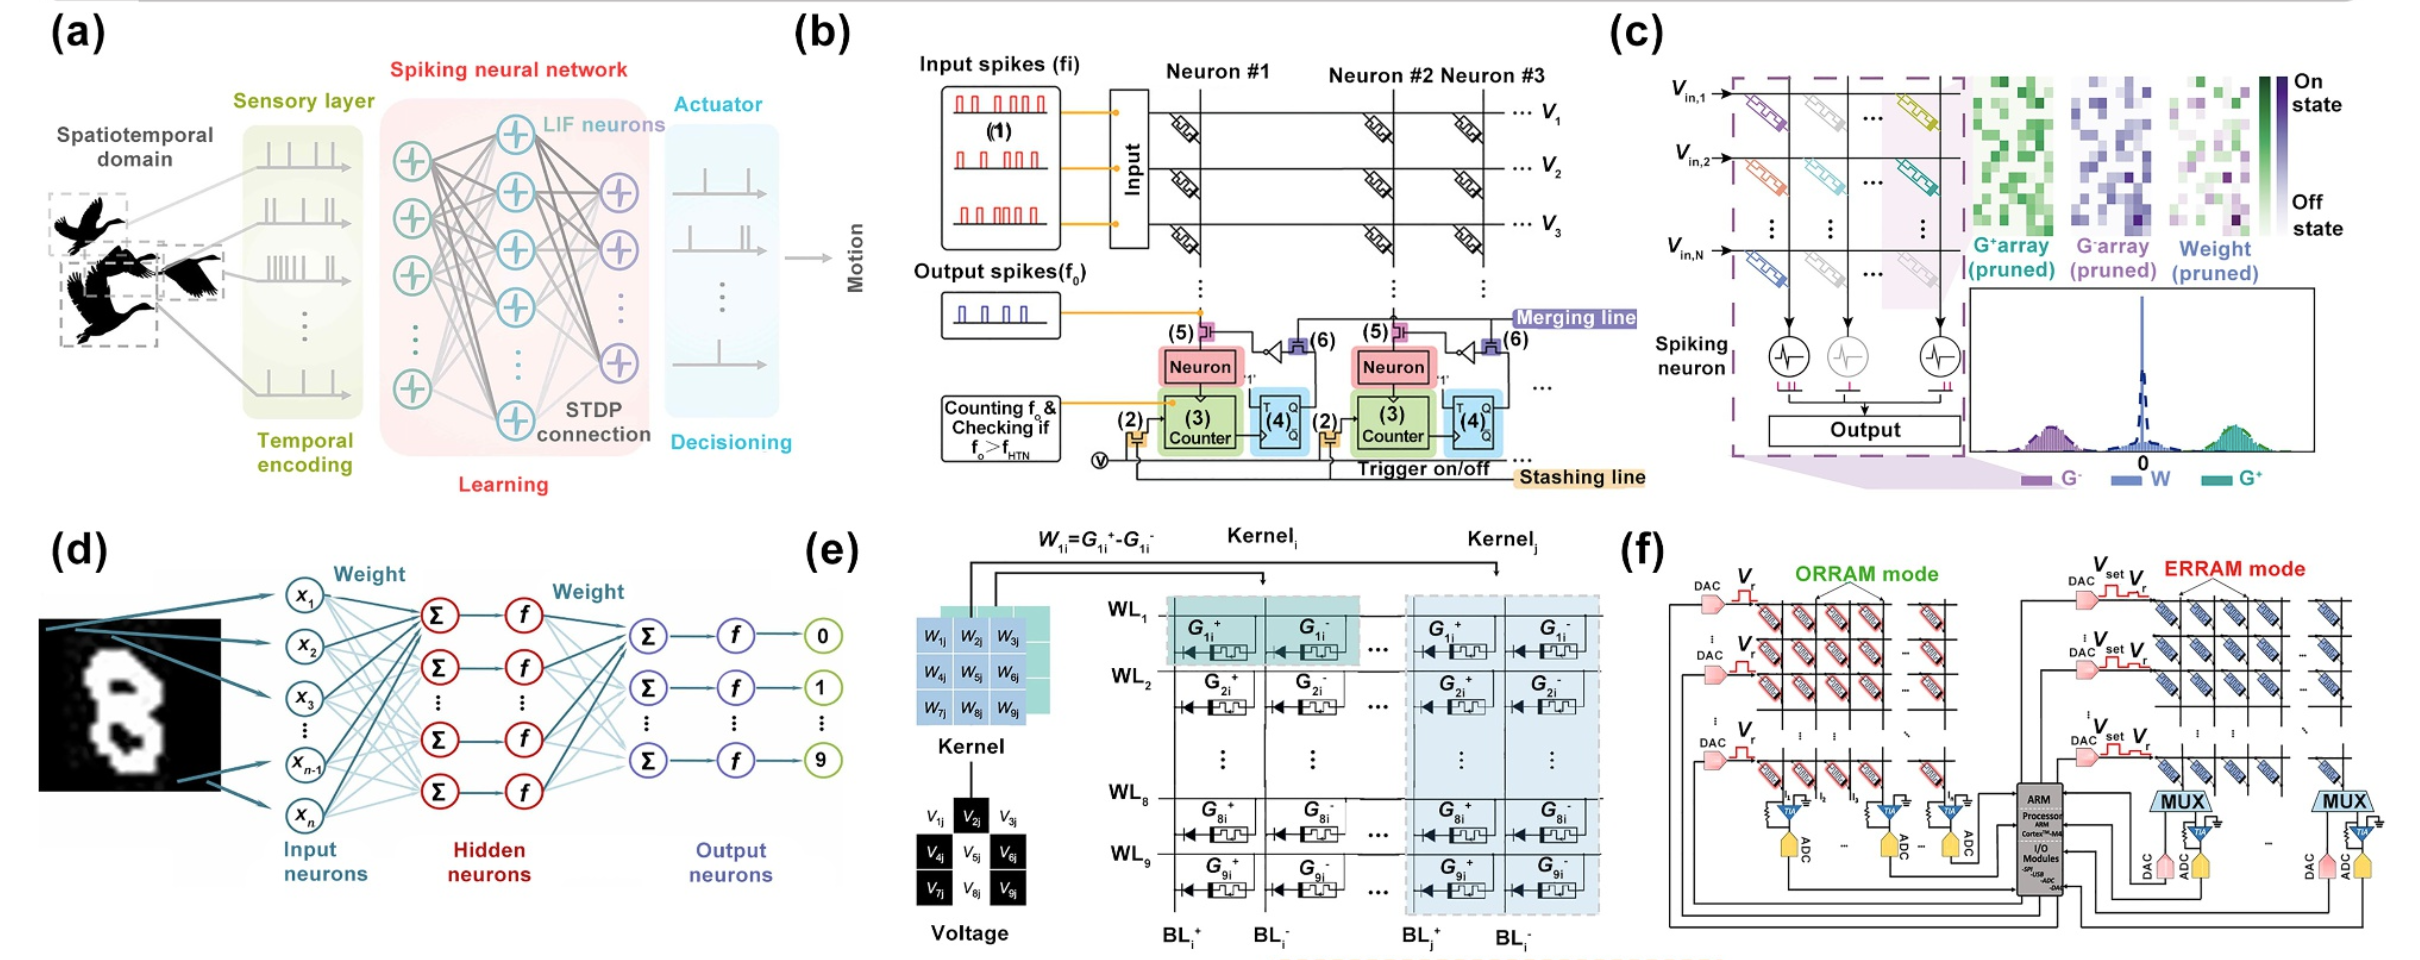
\includegraphics[width=\textwidth]{HardwareSNN.png}
    \caption{Implementaciones en hardware de las SNNs (a) Estructura de una SNN (b) Estrategias de decodificación de los impulsos de salida de un arreglo memristivo, permitiendo la combinación y acumulación de los mismos (c) estructura de una AMC (Analog multiplier-accumulator) (d) implementacion de la prueba MNIST con estructura neuromórfica (e) Convolución de imágenes representando la intensidad de cada pixel como un voltage, y el kernel como valores resistivos en arreglos 1D1M (f) Estructura de multiplicación analógica con recomposición digital. Los ADC y los DACs colaboran con un microcontrolador digital para realizar multiplicacion de matrices analógica. Extraído de  \cite{han2024brain}}
    \label{fig:MEM_IOT}
\end{figure}

\subsection{Celdas estandar neuromórficas propuestas}
Se muestran a continuación algunos de los circuitos analógicos propuestos en este trabajo, para su desarrollo e implementación en VLSI futura. 

\subsubsection{Neurona LIF}
El modelo de neurona LIF (\textit{Leaky Integrate-and-Fire}) simula la dinámica neuronal utilizando un circuito RC con una fuga de corriente constante. Extraído de \cite{math12142267}, el circuito de la neurona LIF se ha modificado levemente para obtener el circuito representado en la Fig.~\ref{fig:LIF}. La corriente de entrada $I_{ext}$ ingresa a la neurona a través de una puerta de transmisión (formada por M1 y M2), cargando el capacitor $C1$ y acumulando tensión en el nodo $v_m$. Se tiene  en cuenta que $M3$ está configurado como diodo (su compuerta y drenador están interconectados), por lo que opera en saturación. La tensión $V_{gs6}$ es entonces proporcional a $v_m$, determinada por la geometría de $M3$ y $M4$. Se puede fijar $V_{gs6} = v_{out}$, lo que significa que este nodo puede utilizarse como la salida de impulsos. La tensión de saturación de $M4$ actúa como la tensión umbral de la neurona LIF que, una vez superada ($v_{out}>v_{th, n}$), la carga almacenada en el capacitor $C1$ fluye a través de $M6$ y $M7$. La señal en $v_{out}$ activa entonces $M6$. Los transistores $M8$ y $M9$ forman un inversor, el cual acondiciona la señal en una forma de onda cuadrada invertida $v_{out,n}$. Se podría añadir un segundo inversor para obtener una señal de impulso cuadrada no invertida $v_{out,rec}$, o alternativamente, se puede utilizar $v_{out}$ directamente. Durante el funcionamiento de la neurona, el capacitor $C1$ se descarga continuamente a una tasa dictada por la corriente que fluye a través de $M4$, la cual depende de $V_{leak}$ (la tensión de compuerta de $M4$). Cada neurona en el circuito emite la señal $v_{out}$ (señal con los impulsos) y $v_{out,n}$.

\begin{figure}[ht]
    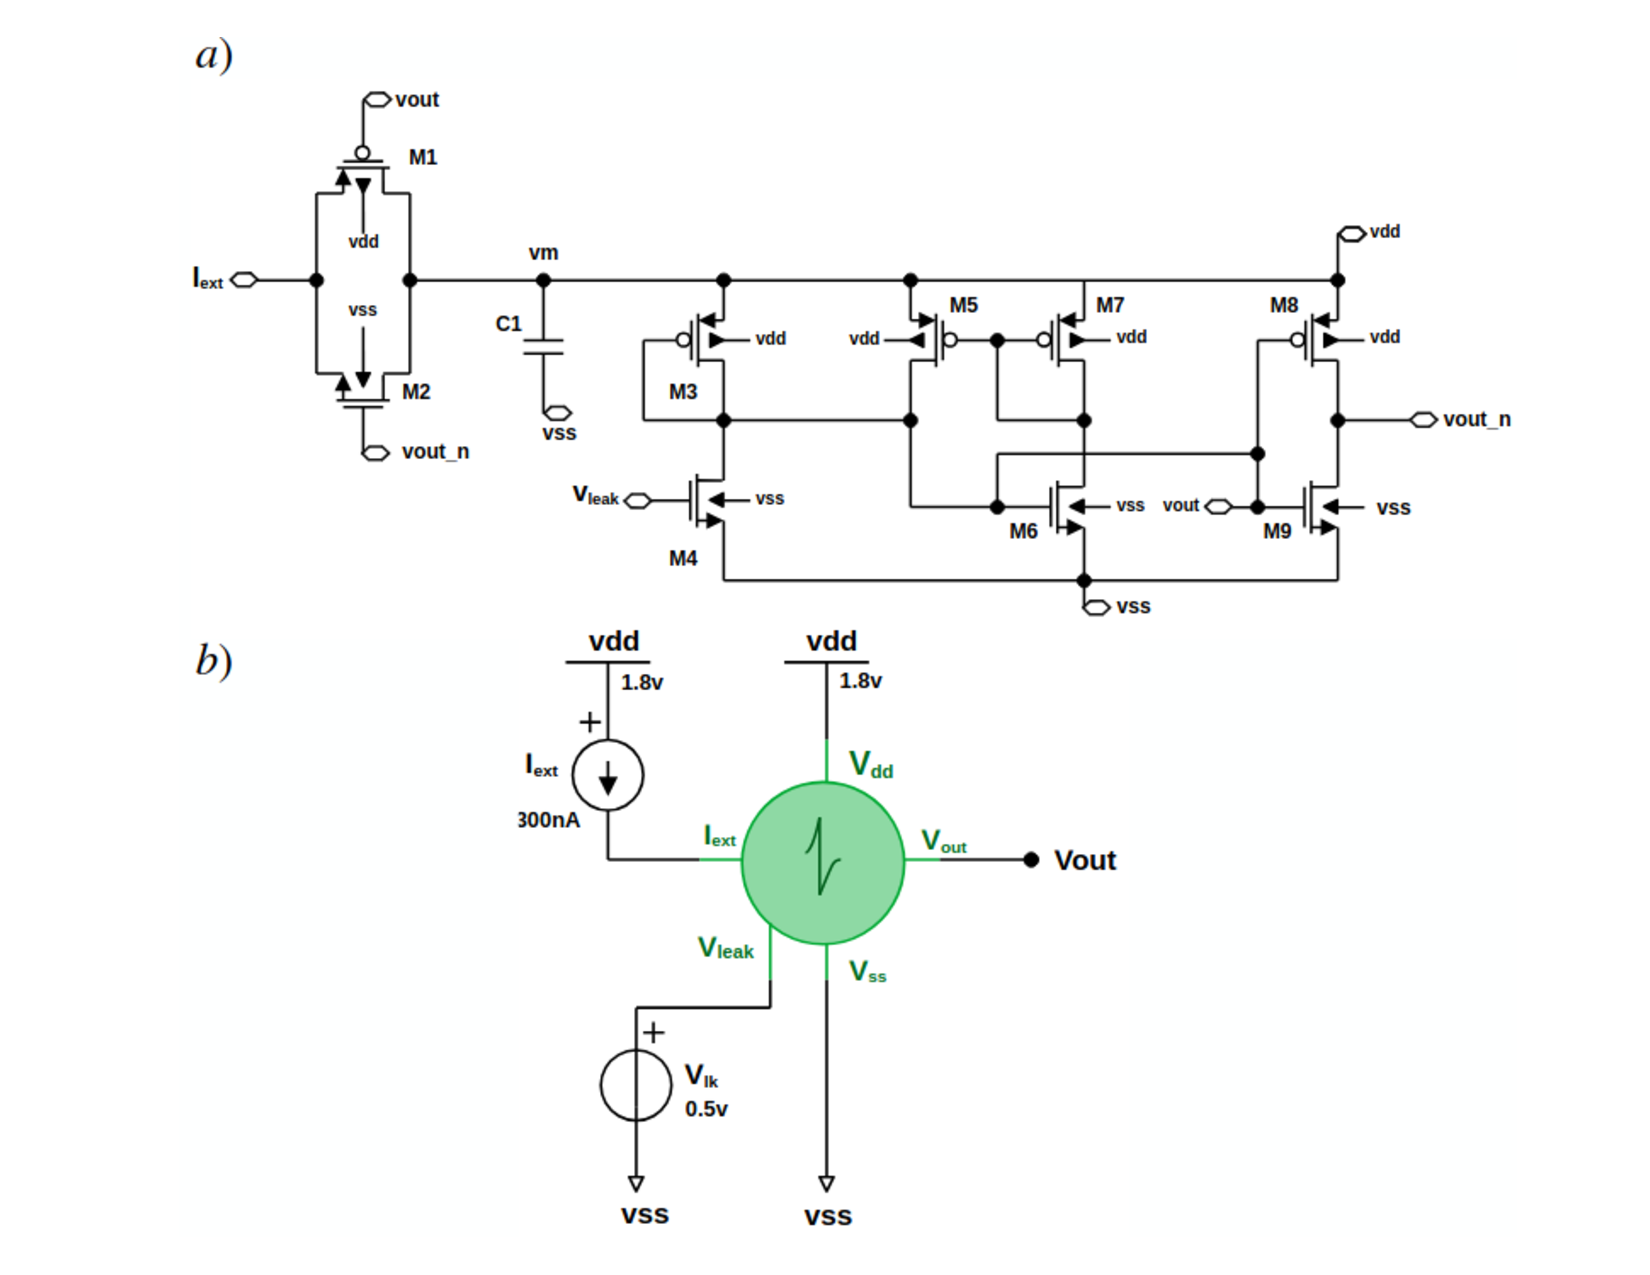
\includegraphics[width=\linewidth]{ul_tun_final1.pdf}
    \caption{{\bf La neurona  de integración y disparo a)El subcircuito CMOS y sus condiciones de operación}\label{fig:LIF}}
\end{figure}

\subsubsection{Sinapsis STDP}

La plasticidad dependiente del tiempo de los impulsos (Spike Time Dependant Plasticity STDP, por sus siglas en inglés) \cite{Salvador2024} modela cómo las sinapsis modifican su fuerza según los tiempos de llegada relativos de los impulsos presinápticos y postsinápticos en el mismo dispositivo~\cite{Yi2023Survey}. La convolución de ambos impulsos produce una diferencia de voltaje entre los dos terminales de un dispositivo con un voltaje de umbral; una vez que se supera este umbral, la conductancia del dispositivo aumenta o disminuye dependiendo de la dirección del flujo de corriente. La Fig.~\ref{fig:synapsestdp} muestra el subcircuito utilizado para implementar las capacidades de aprendizaje STDP en esta red, proporcionando al mismo tiempo la intensidad de excitación necesaria para la programación memristiva y la propagación de corriente hacia adelante. Para este proyecto se propone usar se utiliza un dispositivo memristivo, adaptado de nuestro trabajo previo en \cite{math12142267}. Los memristores son dispositivos eléctricos pasivos cuya conductancia cambia según la corriente que fluye a través de sus terminales, lo que los convierte en candidatos naturales para implementar sinapsis neuronales \cite{Xia2019}. Para el circuito propuesto surgen dos escenarios. Un pico presináptico genera las señales $v_{out,pre}$ y $\bar{v_{out,pre}}$ (las cuales están conectadas a los nodos de compuerta de los transistores $M2$ y $M3$, respectivamente), permitiendo el flujo de corriente desde el electrodo inferior $BE$ hasta el electrodo superior $TE$ del memristor.

Cuando llega un impulso postsináptico, los transistores $M1$ y $M4$ se activan simultáneamente, permitiendo que la corriente fluya desde el electrodo superior hasta el electrodo inferior. Los transistores $M10$, $M11$ y $M12$ actúan como una fuente de corriente hacia adelante para la siguiente capa de neuronas, con una magnitud proporcional a la corriente que fluye a través del memristor. Múltiples fuentes de corriente de este tipo contribuyen de forma continua al nodo de entrada de la $k$-ésima neurona en la siguiente capa, cada una escalada de acuerdo con su valor memristivo correspondiente. Por lo tanto, la corriente de excitación $I_{ext}$ para la $k$-ésima neurona en una capa de $K$ neuronas con $m$ entradas presinápticas viene dada por:

\begin{equation}
    I_{ext, k} = \sum^{j=m}_{j=1} I_{j,k}
    \label{eq:currSumEq}
\end{equation}

\begin{figure}[t]
    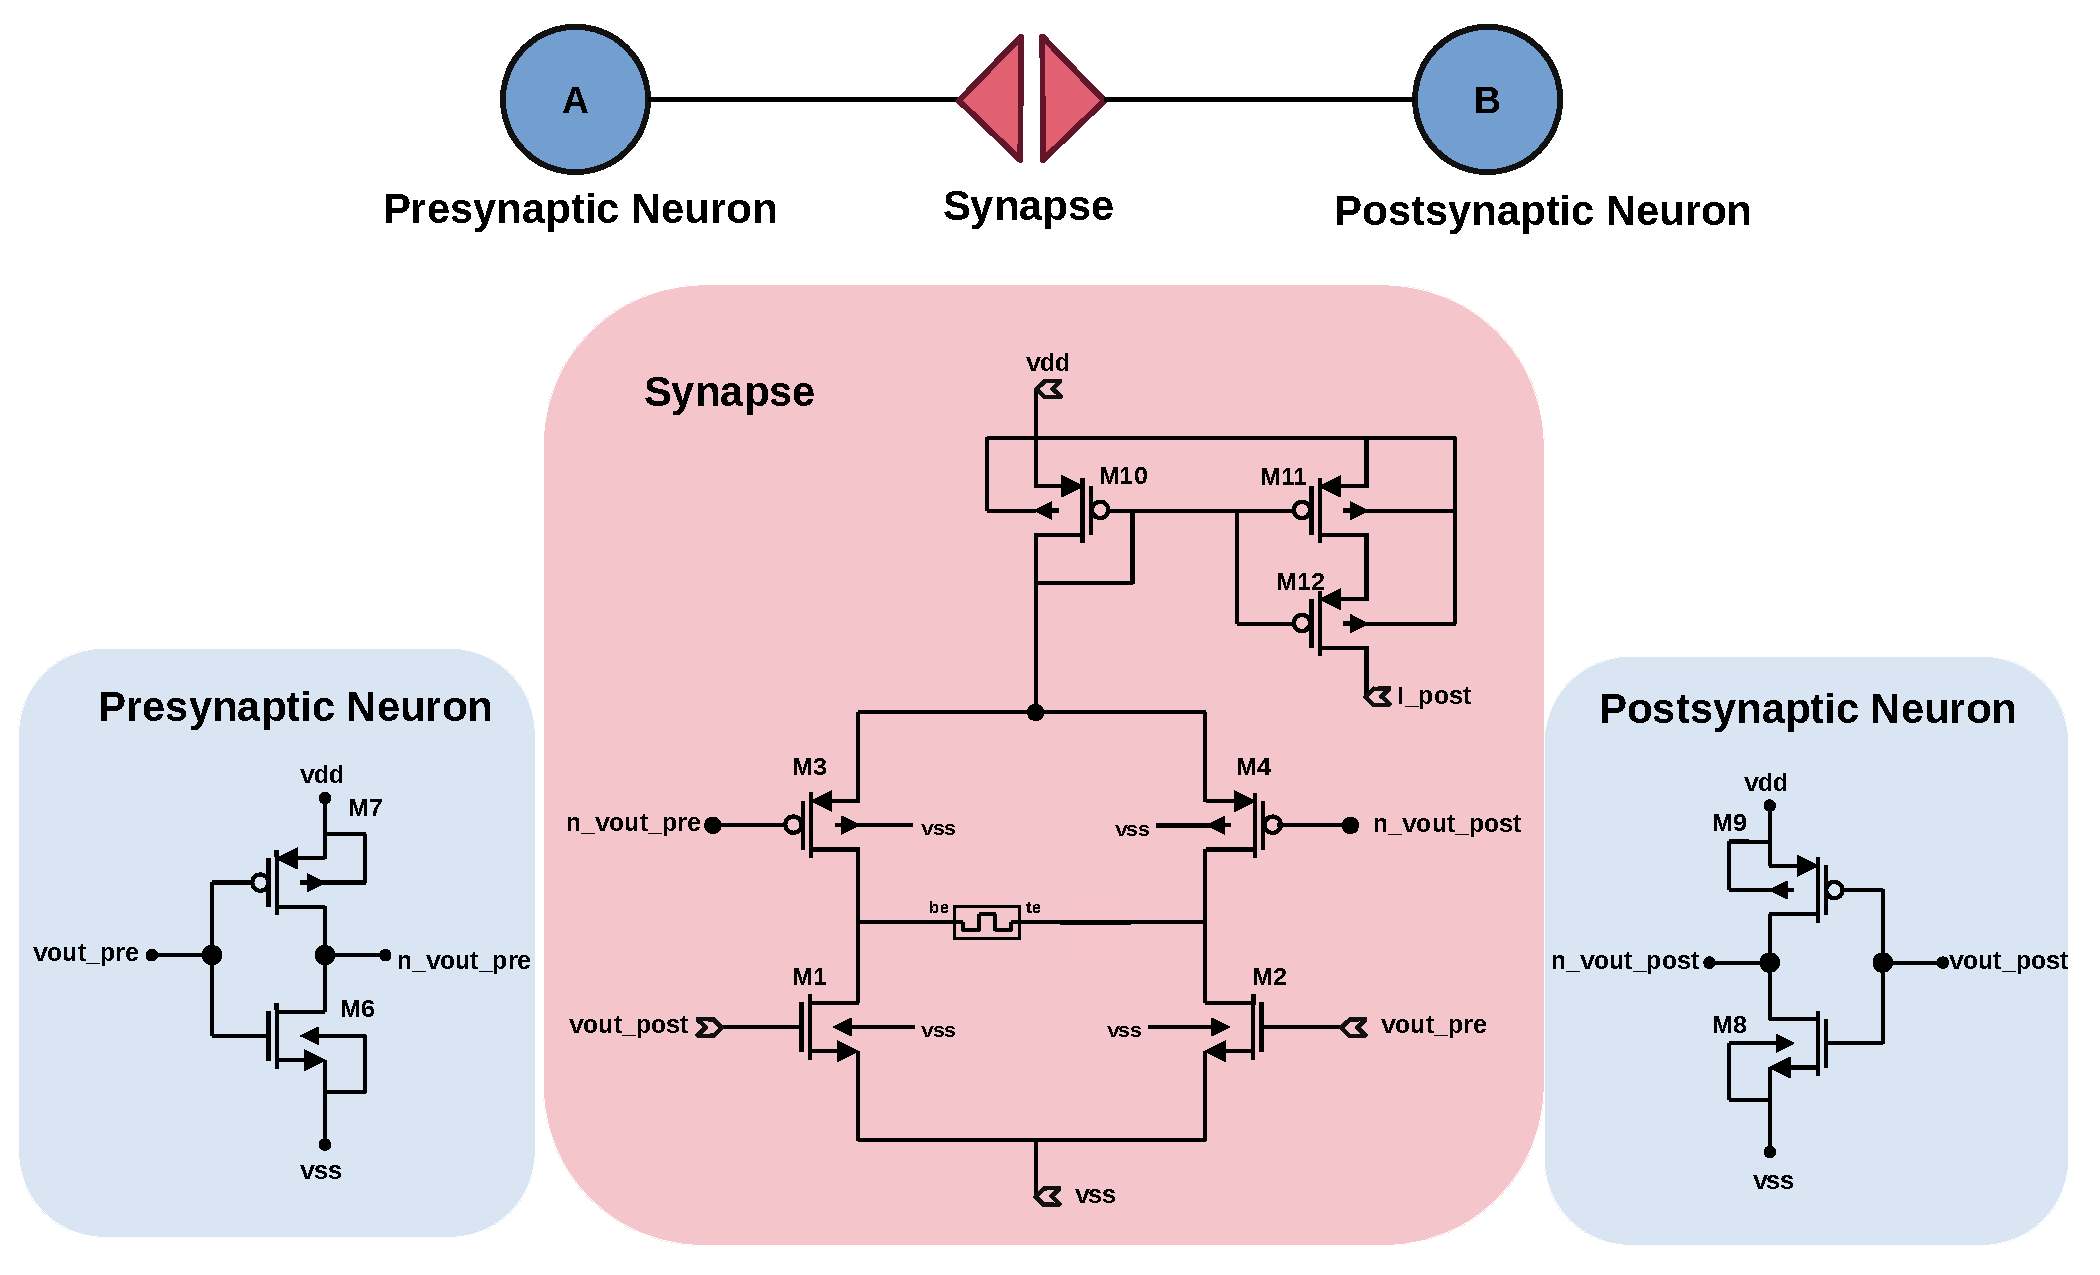
\includegraphics[width=\linewidth]{stdpSynapse_good.pdf}
    \caption{{\bf Proposed Synapse circuit} which enables STDP learning and provides current for the post-synaptic neuron in the next layer. }
    \label{fig:synapsestdp}
\end{figure}

\subsection{Relevancia técnica del proyecto}
\label{subsec:problematics}

Este proyecto toma en cuenta el conocimiento y los avances logrados en el diseño de sistemas neuronales de impulsos con memristores, de autoría propia y original \cite{math12142267, JuarezLora_SNN_IPN, juarez2026snn1, juarez2026snn2}. Para este proyecto se propone el desarrollo de circuitos similares al mostrado en la fig. (\ref{fig:full_stdp_4x2}). Este circuito tiene 4 neuronas de impulso presinápticas y dos de impulso postsinápticas, junto con las respuestas eléctricas de un bloque de aprendizaje, nombrado: STDP 4x2. Este sistema neuronal demuestra los principios de respuesta dinámica de las celdas estándar neuromórficas a desarrollar en este proyecto.

En los resultados gráficos de la fig. (\ref{fig:full_stdp_4x2}), los cuales están basados en el PDK de 180 nm de Global Foundries, se observa que los impulsos de las 4 neuronas presinápticas y los impulsos de las 2 neuronas postsinápticas son atendidos adecuadamente por el bloque STDP 4x2, ajustando dinámicamente el valor de pesos sinápticos como cambios de conductancias memristivas.


\begin{figure}[ht!]
    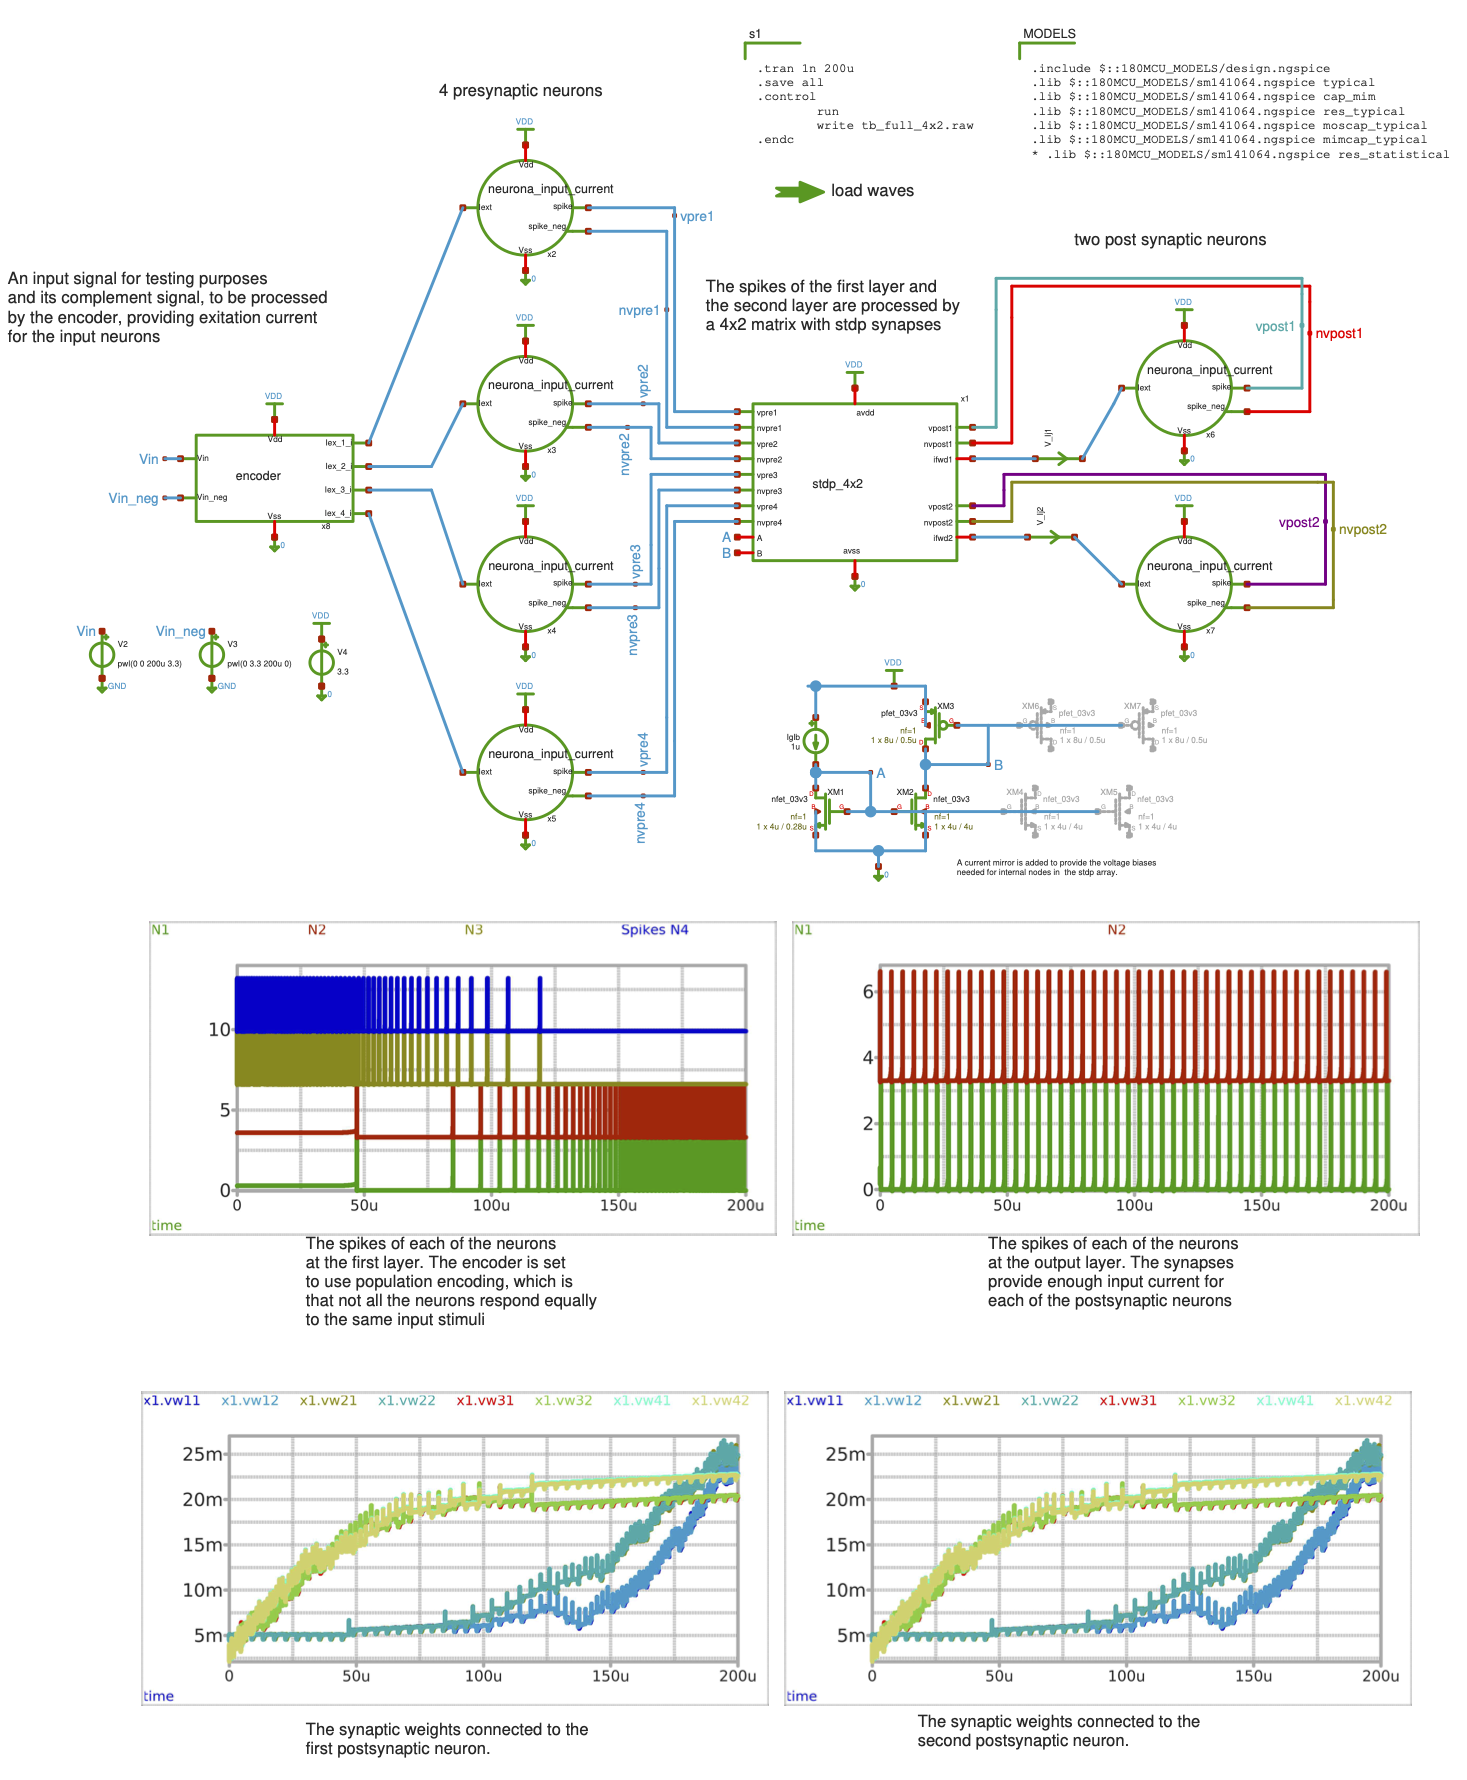
\includegraphics[width=\linewidth]{tb_full_4x2.png}
    \caption{Circuito de red neuronal de impulso implementado en simulacion de dos capas de de neuronas (de 4 y 2 neuronas, respectivamente) completamente conectadas. El bloque  contiene una matriz de subcircuitos STDP que conecta la i-ésima neurona presinpatica con la j-ésima}
    \label{fig:full_stdp_4x2}
\end{figure}

 Si bien, el sistema neuronal de impulsos de la fig.(\ref{fig:full_stdp_4x2}) es viable para su fabricación en silicio, su extensión a prototipos de mediana escala con fines de investigación, educación e innovación debe responder a las 3 preguntas que siguen; marcando la pauta de este proyecto de acuerdo con sus respuestas.


\begin{itemize}
    \item \textbf{¿Cómo automatizar la creación del archivo .SPICE para mayor numero de neuronas o de synapsis?: } Una interfaz grafica es de gran ayuda para circuitos pequeños, ya que toma el dibujo y confecciona el archivo de texto necesario para que el software EDA realice las simulaciones.  Pero la interaccion humano-computadora necesaria para implementar este circuito con $i\times j$ synapsis que conecten $i$ neuronas presynapticas con $j$ neuronas postsynapticas es un reto que puede resolverse con programación. 
    \item \textbf{¿Cómo automatizar la creación del layout neccesario para su fabriación?:} El archivo .SPICE solo sirve para darle al software EDA la abse de datos necesaria que describe a un circuito, pero dicha información debe implementarse en un layout, que son los planos, la topología de cada estructura del circuito en tecnología CMOS micrometrica. Se obtiene al final un archivo .GDSII, el cual es una base de datos que incluye las geometrias cada poligono que resultaran en las máscaras de diseño a imprimirse en silicio. 
    \item \textbf{¿Como se verificara que un diseño de $i\times j$ neuronas automatizado sea viable de fabricación?:} Existen reglas de diseño que los fabricantes de VLSI proveen a los diseñadores (dentro del PDK) que mediante software EDA pueden cumplimentarse. 

    
\end{itemize}


La relevancia técnica de este proyecto se ajusta a las 3 respuestas anteriores, lo que, en síntesis, nos conduce a diseñar circuitos fundamentales de las redes neuronales de impulso y a desarrollar software basado en los esquemas de la industria de semiconductores que automatizan el diseño electrónico; lo que, en conjunto, nos llevaría a desarrollar \textbf{Celdas Estándar Neuromórficas} en plataformas de software libre u open source.


\section{Metodología}

Las 3 respuestas en el apartado anterior (\ref{subsec:problematics}) se traducen en 3 actividades específicas, como sigue:

\begin{itemize}
    \item \textbf{Creación de los archivos .SPICE para la creación de macroceldas}, al ser archivos de texto, es posible automatizar su generación mediante la implementación de código python y uso de cadenas de formato condicional. 
    \item \textbf{Automatización del layout de las subceldas} con el uso de nuevas librerias de software EDA emergentes como glayout y gdsFactory \cite{Hammoud2024, LinanCembrano2024, GDSFactoryWebsite}, que permitirian implementar la creacion de los poligonos de cada subcelda. El marco de integración puede será Librelane \cite{librelane}, la cual, mediante descripción de las conexiones con Verilog, te permite tratar celdas analógicas como bloques, e interconectarlas como diseños digitales. 
    \item \textbf{Verificación de los circuitos con software EDA tipo abierto}: como Magic o Klayout, de código abierto, para verificar las reglas de diseño y eléctricas (DRC, ERC) y realizar las correcciones pertinentes. 
\end{itemize}

De lo anterior, se propone la metodología de ejecución de este proyecto basado en los siguientes puntos (los cuales tambien están contenidos en el diagrama de flujo de la fig. \ref{fig:flowchart_neuromorphic}).

\begin{itemize}
    \item \textbf{Diseño de celdas estándar neuromórficas:} Se realiza trabajo de diseño analógico de las celdas estándar a nivel esquematico (selección de geometrias de los transistores, caracterización de las celdas). Una vez consolidados los diseños, se procede a su implementación en layout. Simulación numérica da certeza del correcto funcionamiento de las celdas por separado
    \item \textbf{Composición de macroceldas:} Se procede a confeccionar capas de neuronas usando descripción estructural con verilog, formato que permitirá automatizar la descripción las conexiones de nodos. Para realizar la sintesis física de las macroceldas, se proporcionan los archivos verilog resultantes a software especializado de síntesis física (i.e. Cadence, Synosis, Librelane) que trata a las celdas neuromórficas como cajas negras, y enrutan correctamente la conexión de puertos. Así también, se procederá con el desarrollo de otras macroceldas como matrices de $i\times j$ sinapsis, que comunican las $i$ neuronas de las capa previa con las $j$ neuronas de la capa anterior. 
    \item \textbf{Verificación de las macroceldas:} El funcionamiento de las macroceldas, tanto de manera individual como en conjunto debe ser verificado para su fabricación. Se procede entonces a hacer el DRC (Revisión de reglas de diseño), ERC (revisión de reglas eléctricas) y la síntesis de la señal de reloj (CTS). 
     \item \textbf{Preparativos para el tapeout:} Se debe entonces preparar la configuración necesaria para incluir el diseño en una oblea multiproyecto (multiproyect wafer). Dicha preparación incluye asignación y preparación de puertos, creacion de bancos de pruebas y documentación pertinente. 
\end{itemize}

El objetivo entonces no es solo tener un layout de una SNN terminada, sino tambien, diseñar la infraestructura de software de automatización que permita sintetizar SNNs en función de los parametros de red (numero de neuronas, numero de capas, etc.). El diagrama de flujo en la fig. \ref{fig:flowchart_neuromorphic} despliega la metodología a seguir de manera resumida
\begin{figure}[htbp]
\centering
\begin{tikzpicture}[node distance=0.5cm, font=\tiny]

% Nodes
\node (start) [startstop] {Inicio};

\node (step1) [process, below=0.2cm of start] {Selección e Implementación\\de celdas neuromórficas\\paramétricas (Neuronas, sinapsis)};

\node (step2) [process, below=0.2cm of step1] {Obtención del layout de cada\\Celda neuromórfica con glayout};

\node (step3) [process, below=0.2cm of step2] {Verificación ERC, DRC\\de las celdas neuromórficas};

\node (dec1) [decision, below=0.3cm of step3] {¿Cumple con\\las reglas de diseño\\del PDK?};

\node (step4) [process, below=0.4cm of dec1] {Uso de Verilog para\\descripción de Macroceldas\\(Capas de neuronas, matrices\\de sinapsis, etc.)};

\node (step5) [process, below=0.2cm of step4] {Composición del layout de las\\macroceldas (glayout/Libelone)};

\node (dec2) [decision, below=0.2cm of step5] {¿Cumple con DRC\\y ERC del PDK?};

\node (step6) [process, below=0.4cm of dec2] {Descripción en Verilog de\\la Macrocelda principal};

\node (step7) [process, below=0.2cm of step6] {Síntesis física con Librelane};

\node (dec3) [decision, below=0.2cm of step7] {¿Síntesis Exitosa?\\(DRC, ERC, CTS)};

\node (step8) [process, below=0.4cm of dec3] {Cierre del trabajo de diseño};

\node (stop) [startstop, below=0.2cm of step8] {Fin};

% Arrows
\draw [arrow] (start) -- (step1);
\draw [arrow] (step1) -- (step2);
\draw [arrow] (step2) -- (step3);
\draw [arrow] (step3) -- (dec1);

\draw [arrow] (dec1) -- node[anchor=west, font=\sffamily\bfseries] {Sí} (step4);
\draw [arrow] (dec1.west) -- ++(-1.8,0) |- node[anchor=south east, near start, font=\sffamily\bfseries] {No} (step2.west);

\draw [arrow] (step4) -- (step5);
\draw [arrow] (step5) -- (dec2);

\draw [arrow] (dec2) -- node[anchor=west, font=\sffamily\bfseries] {Sí} (step6);
\draw [arrow] (dec2.west) -- ++(-1.8,0) |- node[anchor=south east, near start, font=\sffamily\bfseries] {No} (step5.west);

\draw [arrow] (step6) -- (step7);
\draw [arrow] (step7) -- (dec3);

\draw [arrow] (dec3) -- node[anchor=west, font=\sffamily\bfseries] {Sí} (step8);
\draw [arrow] (dec3.west) -- ++(-1.8,0) |- node[anchor=south east, near start, font=\sffamily\bfseries] {No} (step6.west);

\draw [arrow] (step8) -- (stop);

\end{tikzpicture}
\caption{Flujo de diseño para celdas y macroceldas neuromórficas.}
\label{fig:flowchart_neuromorphic}
\end{figure}


\section{Cronograma}
% Incluir una tabla con el cronograma
La tabla \ref{tab:cronograma} incluye un cronograma de actividades que desglosa las fases de investigación, comprendidas a lo largo de 2 años  de investigación. Las actividades a realizar en cada fase están descritas a continuación:

\begin{itemize}
    \item \textbf{Fase 1 (Febrero a Julio del 2027):} En esta fase se evaluará en el estado del arte la tecnologías disponibles en el desarrollo de semiconductores, que ofrezcan las capacidades en FEOL (Front end of the Line)  para nuestros diseños. A su vez, se diseñaran simulaciones numericas en software especializado de codigo abierto para mostrar resultados preeliminares de una estructura de SNN analogica de proposito general. (Entregable: Informe del edo. del arte: un diseño preeliminar en esquemático, simulaciones pre-layout, posibles fabricantes + cotizaciones de fabricación, documento de requerimentos del producto minimo viable)
    \item \textbf{Fase 2 (Agosto del 2027 a Enero del 2028):}  En esta fase, se desarrollaran los layouts, simulación post-layout y verificación funcional de las celdas estándar neuromórficas. Se realizarán los correspondientes análisis energéticos, de verificación y funcionales que garanticen el correcto funcionamiento del dispositivo una vez fabricado.  Al final de esta fase se deberá contar un archivo GDSII de cada una de las celdas neuromórficas propuestas en(Entregable: Informe de actividades: - Diseño del circuito en esquematico - Implementación en layout - Layout vs Schematic del circuito - Simulación post-layout - Carpeta con la estructura de archivos .v, .mag)
    \item \textbf{Fase 3 (Febrero del 2028 a Julio del 2028):} Integración de macroceldas. Usando las subceldas y software especializado de sintesis física de software libre, se trabajara en la configuración y composición de macroceldas para la red, como capas de neuronas, arreglos de sinapsis stdp, codificadores de entrada, decodificadores de salida. Estas macroceldas daran pie a la construcción de la SNN analógica, completa. Su composición requiere la creación de archivos .v para describir la estructura de conexión de nodos, y la creación de archivos de configuración como para el software de síntesis física. (Entregable: archivo .gdsII del layout de la red SNN , scripts de automatización de layout usando Librelane)
    \item \textbf{Fase 4 (Agosto del 2028 a Enero del 2029):} Para esta fase se enfocará en recopilar, procesar y reportar los resultados obtenidos, con la finalidad de generar los reportes académicos correspondientes (artículos, ponencias, carteles, presentaciones para congresos). Se revisara el desempeño del dispositivo resultante mediante simulaciones numericas con miras a realizar un segundo prototipo con mejoras en desempeño energético y escalabilidad a trabajo futuro, que permita implementar soluciones de IA de mayor tamaño. (Entregable: Reporte final de actividades: - Diseños de circuito finales, - Reportes de desempeño - Discusión - Conclusiones y trabajo futuro) 
\end{itemize}

\section{Actividades complementarias}

Debido a la naturaleza del proyecto, a lo largo de las fases pronosticadas, se tiene la capacidad de realizar las siguientes tareas complementarias:

\begin{itemize}
    \item Capacitación y formación de estudiantes de pregrado y posgrado en el área de desarrollo de control automático, semiconductores, inteligencia artificial  mediante cursos y/o talleres.
    \item Participación con grupos de estudiantes de posgrado y pregado en iniciativas de concurso de desarrollo de dispositivos semiconductores (Chipathon) organizados por instituciones normativas en diseño VLSI, como IEEE.
    \item Publicación de resultados preliminares y finales en revistas con indice JCR, especializadas en telecomunicaciones, procesamiento de señales, cómputo neuromórfico, entre otros.
\end{itemize}



\begin{table}[h!]
    \centering
    \caption{Cronograma de Actividades (2027--2029)}
    \label{tab:cronograma}
    \renewcommand{\arraystretch}{1.2}
    \setlength{\extrarowheight}{1pt}
    \begin{tabularx}{\textwidth}{|>{\centering\arraybackslash}X|*{8}{>{\centering\arraybackslash}X|}}
        \hline
        \textbf{Fase} & \textbf{Feb--Abr 2027} & \textbf{May--Jul 2027} & \textbf{Ago--Oct 2027} & \textbf{Nov 2027--Ene 2028} & \textbf{Feb--Abr 2028} & \textbf{May--Jul 2028} & \textbf{Ago--Oct 2028} & \textbf{Nov 2028--Ene 2029} \\
        \hline
        \textbf{Fase 1} & X & X & & & & & & \\
        \hline
        \textbf{Fase 2} & & X & X & X & & & & \\
        \hline
        \textbf{Fase 3} & & & & X & X & X & & \\
        \hline
        \textbf{Fase 4} & & & & & & & X & X \\
        \hline
    \end{tabularx}
\end{table}

\section{Recursos}
\subsection{Recursos materiales}
% Materiales necesarios
\begin{itemize}
    \item Equipo de cómputo y Área de trabajo (oficina)
    \item Acceso a las revistas, acervos y repositorios de investigación cientifica como los son IEEEXplore, Nature, etc. 
    \item Acceso a equipo de laboratorio para caracterización de circuitos semiconductores (Osciloscopio, generador de señales, analizador de redes, etc)
\end{itemize}

\subsection{Recursos humanos}
% Personal requerido
A lo largo del desarrollo del proyecto, se espera contar con estudiantes de licenciatura y de posgrado, que colaboren con el diseño, verificación, análisis y síntesis de distintos subcomponentes del hardware implementado, asi como con los bancos de prueba de control de lazo cerrado pertinentes.



\section{Resultados Esperados}
% Posibles hallazgos e impacto
\begin{itemize}
    \item  Formación de recursos humanos en cómputo analógico, procesamiento de señales y desarrollo VLSI, mediante talleres y seminarios a lo largo de la estancia posdoctoral
    \item Diseñode prototipos de circuitos CMOS para implentación de algoritmos de aprendizaje automático en bajo consumo. 
    \item Publicación de los resultados teóricos y prácticos del proyecto en revistas de investigación.
    \end{itemize}
    
\section{Referencias Bibliográficas}


\begin{thebibliography}{99}

\bibitem{Zanatta2024}
L.~Zanatta, F.~Barchi, S.~Manoni, S.~Tolu, A.~Bartolini, and A.~Acquaviva,
``Exploring spiking neural networks for deep reinforcement learning in robotic tasks,''
\emph{Scientific Reports}, vol.~14, no.~1, p.~30648, 2024.
[Online]. Available: \url{https://doi.org/10.1038/s41598-024-77779-8}

\bibitem{11534092}
M.~Shatta, S.~Nassif, G.~Zervakis, and M.~B. Tahoori,
\newblock ``AML-K: An Analog Machine Learning Accelerator for K-Means at the Edge with Hardware-Software Co-Optimization,''
\newblock {\em IEEE Transactions on Circuits and Systems for Artificial Intelligence}, pp.~1--14, 2026.

\bibitem{Sutton}
R.~S.~Sutton and A.~G.~Barto,
\emph{Reinforcement Learning: An Introduction},
2nd~ed.
Cambridge, MA, USA: MIT Press, 2018.
[Online]. Available: \url{https://web.stanford.edu/class/psych209/Readings/SuttonBartoIPRLBook2ndEd.pdf}


\bibitem{Morcos2019}
B.~Morcos,
``NengoFPGA: an FPGA Backend for the Nengo Neural Simulator,''
M.S.~thesis, Dept. of Electrical and Computer Engineering, University of Waterloo, Waterloo, ON, Canada, Aug.~2019. [Online]. Available: \url{http://hdl.handle.net/10012/14923}


\bibitem{Zhang2022}
X.~Zhang, Y.~Zeng, Y.~Lin, and L.~Zhou,
``Transfer modeling of 1T1R crossbar arrays with line resistances based on matrix algebra method,''
\emph{Solid-State Electronics}, 189, p.~108220, 2022.
[Online]. Available: \url{https://www.sciencedirect.com/science/article/pii/S003811012100263X}
doi: \href{https://doi.org/10.1016/j.sse.2021.108220}{10.1016/j.sse.2021.108220}

\bibitem{Vlasov2023}
D.~Vlasov, A.~Minnekhanov, R.~Rybka, Y.~Davydov, A.~Sboev, A.~Serenko, A.~Ilyasov, and V.~Demin,
``Memristor-based spiking neural network with online reinforcement learning,''
\emph{Neural Networks}, 166, pp.~512--523, 2023.
[Online]. Available: \url{https://www.sciencedirect.com/science/article/pii/S0893608023003891}
doi: \href{https://doi.org/10.1016/j.neunet.2023.07.031}{10.1016/j.neunet.2023.07.031}

\bibitem{Sun2022}
Z.~Sun and D.~Ielmini,
``Invited tutorial: Analog matrix computing with crosspoint resistive memory arrays,''
\emph{IEEE Transactions on Circuits and Systems II: Express Briefs}, vol.~69, no.~7, pp.~3024--3029, 2022.
doi: \href{https://doi.org/10.1109/TCSII.2022.3174920}{10.1109/TCSII.2022.3174920}

\bibitem{11576581}
F.~B. Guo, K.~T. Ho, A.~Vladimirescu, and B.~Nikoli\'{c},
\newblock ``What Can Machine Learning Do for Circuits?: Practical findings from principled machine learning applications,''
\newblock {\em IEEE Solid-State Circuits Magazine}, vol.~18, no.~2, pp.~83--92, 2026.

\bibitem{Parmar2023}
V.~Parmar, S.~K.~Kingra, S.~Negi, and M.~Suri,
``Analysis of VMM computation strategies to implement BNN applications on RRAM arrays,''
\emph{APL Machine Learning}, vol.~1, no.~2, p.~026108, Apr.~2023.
[Online]. Available: \url{https://doi.org/10.1063/5.0139583}
doi: \href{https://doi.org/10.1063/5.0139583}{10.1063/5.0139583}

\bibitem{Yi2023}
H.~Zheng and Y.~(C.)~Yi,
``Spiking neural encoding and hardware implementations for neuromorphic computing,''
in \emph{Neuromorphic Computing}, Y.~(C.)~Yi and H.~An, Eds. London, U.K.: IntechOpen, 2023, ch.~7.
doi: \href{https://doi.org/10.5772/intechopen.113050}{10.5772/intechopen.113050}

\bibitem{Pereira2023}
M.~E.~Pereira, E.~Carlos, E.~Fortunato, R.~Martins, P.~Barquinha, and A.~Kiazadeh,
``Amorphous oxide semiconductor memristors: Brain-inspired computation,''
in \emph{Advanced Memory Technology: Functional Materials and Devices}. 
London, U.K.: Royal Society of Chemistry, Oct.~2023.
doi: \href{https://doi.org/10.1039/BK9781839169946-00431}{10.1039/BK9781839169946-00431}

\bibitem{librelane}
LibreLane Developers. (2026). \textit{LibreLane: An open-source digital ASIC implementation flow}. GitHub repository. https://github.com/librelane/librelane

\bibitem{Tapson2013}
J.~C.~Tapson, G.~K.~Cohen, S.~Afshar, K.~M.~Stiefel,
Y.~Buskila, R.~M.~Wang, T.~J.~Hamilton, and A.~van~Schaik,
``Synthesis of neural networks for spatio-temporal spike pattern recognition and processing,''
\emph{Frontiers in Neuroscience}, vol.~7, Art.~153, 2013.
[Online]. Available: \url{https://www.frontiersin.org/journals/neuroscience/articles/10.3389/fnins.2013.00153}
doi: \href{https://doi.org/10.3389/fnins.2013.00153}{10.3389/fnins.2013.00153}

\bibitem{Liu2022}
X.~Liu and Z.~Zeng,
``Memristor crossbar architectures for implementing deep neural networks,''
\emph{Complex \& Intelligent Systems}, vol.~8, no.~2, pp.~787--802, Apr.~2022.
[Online]. Available: \url{https://doi.org/10.1007/s40747-021-00282-4}
doi: \href{https://doi.org/10.1007/s40747-021-00282-4}{10.1007/s40747-021-00282-4}

\bibitem{Liu2023}
F.~Liu, L.~Zhang, J.~Yang, and W.~Wu,
``Adaptive Fuzzy Population Coding Method for Spiking Neural Networks,''
\textit{International Journal of Fuzzy Systems},
vol.~25, no.~2, pp.~670--683, 2023.
doi: \href{https://doi.org/10.1007/s40815-022-01395-9}{10.1007/s40815-022-01395-9}.

\bibitem{Yi2023Survey}
Z.~Yi, J.~Lian, Q.~Liu, H.~Zhu, D.~Liang, and J.~Liu,
``Learning rules in spiking neural networks: A survey,''
\emph{Neurocomputing}, vol.~531, pp.~163--179, 2023.
doi: \href{https://doi.org/10.1016/j.neucom.2023.02.026}{10.1016/j.neucom.2023.02.026}.

\bibitem{Hazan2021}
A.~Hazan and E.~T.~Ezra Tsur,
``Neuromorphic analog implementation of Neural Engineering Framework-inspired spiking neuron for high-dimensional representation,''
\emph{Frontiers in Neuroscience}, vol.~15, 2021.
[Online]. Available: \url{https://www.frontiersin.org/journals/neuroscience/articles/10.3389/fnins.2021.627221}
doi: \href{https://doi.org/10.3389/fnins.2021.627221}{10.3389/fnins.2021.627221}

\bibitem{Feinberg2021}
B.~Feinberg, R.~Wong, T.~P.~Xiao, C.~H.~Bennett, J.~N.~Rohan, E.~G.~Boman, M.~J.~Marinella, S.~Agarwal, and E.~Ipek,
``An Analog Preconditioner for Solving Linear Systems,''
in \emph{Proc. IEEE Int. Symp. High-Performance Computer Architecture (HPCA)}, 2021, pp.~761--774.
doi: \href{https://doi.org/10.1109/HPCA51647.2021.00069}{10.1109/HPCA51647.2021.00069}

\bibitem{Mayr2014}
C.~G.~Mayr, J.~Partzsch, M.~Noack, and R.~Schüffny,
``Configurable analog-digital conversion using the neural engineering framework,''
\emph{Frontiers in Neuroscience}, vol.~8, 2014.
doi: \href{https://doi.org/10.3389/fnins.2014.00201}{10.3389/fnins.2014.00201}.

\bibitem{Xia2019}
Q.~Xia and J.~J.~Yang,
``Publisher Correction: Memristive crossbar arrays for brain-inspired computing,''
\textit{Nature Materials},
vol.~18, no.~4, pp.~309--323, 2019.
doi: \href{https://doi.org/10.1038/s41563-019-0357-9}{https://doi.org/10.1038/s41563-019-0357-9}.
\bibitem{9937639}
M.~Tian, J.~Lu, H.~Gao, H.~Wang, J.~Yu, and C.~Shi,
``A Lightweight Spiking GAN Model for Memristor-centric Silicon Circuit with On-chip Reinforcement Adversarial Learning,''
in \textit{2022 IEEE International Symposium on Circuits and Systems (ISCAS)}, 2022, pp. 3388--3392, doi: 10.1109/ISCAS48785.2022.9937639.

\bibitem{Niedermeier_2025}
L.~Niedermeier, N.~Dutt, and J.~L.~Krichmar,
``An integrated toolbox for creating neuromorphic edge applications,''
\textit{Neuromorphic Computing and Engineering},
vol.~5, no.~1, p.~014003, Jan. 2025.
doi: \href{https://doi.org/10.1088/2634-4386/adad0f}{10.1088/2634-4386/adad0f}.

\bibitem{TorresChavez2025}
G.~S.~Torres-Ch\'avez, L.~A.~Vallejo-Mora, J.~A.~Ju\'arez-Lora, and H.~Molina-Lozano,
``Noise Suppression in ECG Signals Based on Izhikevich’s Spiking Neuron,''
in \emph{Proc. IEEE Latin American Conference on Computational Intelligence (LA-CCI)},
2025, pp.~1--6.
doi:~10.1109/LA-CCI66231.2025.11270437.

\bibitem{Jebali2024}
F.~Jebali, A.~Majumdar, C.~Turck, K.-E.~Harabi, M.-C.~Faye, E.~Muhr,
J.-P.~Walder, O.~Bilousov, A.~Michaud, E.~Vianello, T.~Hirtzlin,
F.~Andrieu, M.~Bocquet, S.~Collin, D.~Querlioz, and J.-M.~Portal,
``Powering AI at the edge: A robust, memristor-based binarized neural network
with near-memory computing and miniaturized solar cell,''
\emph{Nature Communications}, vol.~15, no.~1, p.~741, 2024.
doi:~10.1038/s41467-024-44766-6.

\bibitem{caravel_fulgor_opamp}
D.~Hernando, ``\textit{caravel\_fulgor\_opamp: Test Chip General Purpose OpAmp using Skywater SKY130 PDK},'' GitHub repository, Dec.~2020. [Online]. Available: \url{https://github.com/diegohernando/caravel_fulgor_opamp}

\bibitem{Hammoud2024}
A.~Hammoud, C.~Goyal, S.~Pathen, A.~Dai, A.~Li, G.~Kielian, and M.~Saligane,
``Human language to analog layout using GLayout layout automation framework,''
in \emph{Proc. 2024 ACM/IEEE 6th Symposium on Machine Learning for CAD (MLCAD)}, 
pp.~1--7, 2024.
doi: \href{https://doi.org/10.1109/MLCAD62225.2024.10740211}{10.1109/MLCAD62225.2024.10740211}.

\bibitem{Valdes_2024}
Valdés, C. (2024). Cadena de suministro de semiconductores. \textit{Entrelíneas}, 3(2), e030204. https://doi.org/10.56368/Entrelineas324

\bibitem{LinanCembrano2024}
G.~Linán-Cembrano, N.~Lourenço, N.~Horta, and J.~M.~de~la~Rosa,
``Design automation of analog and mixed-signal circuits using neural networks—A tutorial brief,''
\emph{IEEE Transactions on Circuits and Systems II: Express Briefs}, 
vol.~71, no.~3, pp.~1677--1682, 2024.  
doi: \href{https://doi.org/10.1109/TCSII.2023.3323886}{10.1109/TCSII.2023.3323886}.

\bibitem{Li2023}
Z.~Li and A.~C.~Carusone,
``Design and optimization of low-dropout voltage regulator using relational graph neural network and reinforcement learning in open-source SKY130 process,''
in \emph{Proceedings of the 2023 IEEE/ACM International Conference on Computer Aided Design (ICCAD)}, 
pp.~01--09, 2023.  
doi: \href{https://doi.org/10.1109/ICCAD57390.2023.10323720}{10.1109/ICCAD57390.2023.10323720}.


\bibitem{Salvador2024}
E.~Salvador, R.~Rodriguez, E.~Miranda, J.~Martin-Martinez, A.~Rubio,
V.~Ntinas, G.~Ch.~Sirakoulis, A.~Crespo-Yepes, and M.~Nafria,
\newblock ``Stochastic resonance in HfO$_2$-based memristors: Impact of external noise on the binary STDP protocol,''
\newblock \emph{IEEE Transactions on Electron Devices}, vol.~71, no.~9,
pp.~5761--5766, Sep.~2024.
\newblock doi:~10.1109/TED.2024.3435173.


\bibitem{Marrero2024NEF}
D.~Marrero, J.~Kern, and C.~Urrea,
``A Novel Robotic Controller Using Neural Engineering Framework-Based Spiking Neural Networks,''
\emph{Sensors}, vol.~24, no.~2, art.~491, 2024.
doi: \href{https://doi.org/10.3390/s24020491}{10.3390/s24020491}.

\bibitem{Snyder2024Lava}
S.~Snyder, S.~Risbud, and M.~Parsa,
``Asynchronous Neuromorphic Optimization in Lava,''
in \emph{Proceedings of the Great Lakes Symposium on VLSI 2024 (GLSVLSI '24)}, 
Clearwater, FL, USA, 2024, pp.~776--778.
doi: \href{https://doi.org/10.1145/3649476.3660383}{10.1145/3649476.3660383}.


\bibitem{math12142267}
A.~Juarez-Lora, V.~H.~Ponce-Ponce, H.~Sossa-Azuela, O.~Espinosa-Sosa, and E.~Rubio-Espino,
``Building an Analog Circuit Synapse for Deep Learning Neuromorphic Processing,''
\textit{Mathematics},
vol.~12, no.~14, article~2267, 2024.
doi: \href{https://doi.org/10.3390/math12142267}{10.3390/math12142267}.

\bibitem{JuarezLora_SNN_IPN}
A.~Juarez-Lora, \emph{SNN\_IPN: Spiking Neural Network implementation repository}. GitHub, 2025. Available at: https://github.com/AlejandroJuarezLora/SNN\_IPN


\bibitem{tinytapeout_LIF_neuron}
H.~Xia,
\newblock \emph{458 AFM\_LIF: Hardware implementation of approximate computing based LIF neuron model},
\newblock Tiny Tapeout project page, 2025.
\newblock Available at: \url{https://tinytapeout.com/chips/ttsky25a/tt_um_LIF_neuron}
\newblock (accessed December 15, 2025).


\bibitem{Kudithipudi2025}
D.~Kudithipudi, C.~Schuman, C.~M.~Vineyard, T.~Pandit, C.~Merkel, R.~Kubendran,
J.~B.~Aimone, G.~Orchard, C.~Mayr, R.~Benosman, J.~Hays, C.~Young,
C.~Bartolozzi, A.~Majumdar, S.~G.~Cardwell, M.~Payvand, S.~Buckley,
S.~Kulkarni, H.~A.~Gonzalez, G.~Cauwenberghs, C.~S.~Thakur,
A.~Subramoney, and S.~Furber,
\newblock ``Neuromorphic computing at scale,''
\newblock \emph{Nature}, vol.~637, no.~8047, pp.~801--812, Jan.~2025.
\newblock doi:~10.1038/s41586-024-08253-8.


\bibitem{Hammoud2024GLayout}
A.~Hammoud, C.~Goyal, S.~Pathen, A.~Dai, A.~Li, G.~Kielian, and M.~Saligane,
``Human Language to Analog Layout Using GLayout Layout Automation Framework,''
in \emph{Proceedings of the 2024 ACM/IEEE International Symposium on Machine Learning for CAD (MLCAD~'24)},
Salt Lake City, UT, USA, 2024, Article~33, 7~pages.
doi:~\href{https://doi.org/10.1145/3670474.3685971}{10.1145/3670474.3685971}.


\bibitem{Zhang2026}
Q.~Zhang, J.~Guo, C.~Jiang, J.~Yao, and Z.~Tao,
\newblock ``The shift to data-driven microelectronics: machine learning for MOSFET modeling, design, and reliability,''
\newblock {\em Journal of Computational Electronics}, vol.~25, no.~3, 2026.

\bibitem{Jespers_Murmann_2017}
P.~G.~A. Jespers and B.~Murmann, \emph{Systematic Design of Analog CMOS Circuits: Using Pre-Computed Lookup Tables}.
\newblock Cambridge: Cambridge University Press, 2017.

\bibitem{Hammoud2023OpenFASOC}
A.~Hammoud, V.~Shankar, R.~Mains, T.~Ansell, J.~Matres, and M.~Saligane,
``OpenFASOC: An Open Platform Towards Analog and Mixed-Signal Automation and Acceleration of Chip Design,''
in \emph{Proceedings of the 2023 International Symposium on Devices, Circuits and Systems (ISDCS)},
Higashihiroshima, Japan, 2023, pp.~01--04.
doi:~\href{https://doi.org/10.1109/ISDCS58735.2023.10153547}{10.1109/ISDCS58735.2023.10153547}.

\bibitem{GDSFactoryWebsite}
GDSFactory, ``GDSFactory: All-in-one software solutions for chip design,'' Website, 2025. [Online]. Available: \url{https://gdsfactory.com}. Accessed: Feb. 3, 2026.

\bibitem{Zuo2025}
P.~Zuo, Q.~Wang, Y.~Luo, R.~Xie, S.~Wang, Z.~Cheng, L.~Bao, Z.~Wang, Y.~Cai, R.~Huang, and Z.~Sun,  
“Precise and scalable analogue matrix equation solving using resistive random-access memory chips,”  
\emph{Nature Electronics}, vol.~8, no.~12, pp.~1222--1233, Dec.~2025.  
doi: 10.1038/s41928-025-01477-0.

\bibitem{ngspice44}
H.~Vogt, G.~Atkinson, and P.~Nenzi,
\emph{Ngspice User's Manual, Version 44},
ngspice Project, SourceForge, 2024.
Available at:
\url{https://ngspice.sourceforge.io/docs/ngspice-44-manual.pdf}

\bibitem{skywater_pdk_docs}
SkyWater Technology Foundry,
\textit{SkyWater SKY130 PDK Documentation},
\url{https://skywater-pdk.readthedocs.io/en/main/index.html},
accessed February 5, 2026.


\bibitem{juarez2026snn1}
A.~Juarez-Lora, ``tb 2x1,'' GitHub repository: SNN\_IPN, 2026. [Online]. Available: \url{https://github.com/AlejandroJuarezLora/SNN_IPN/blob/main/sim_results/triangular_2x1/tb_2x1_triang_rew_at_neuron.pdf}. [Accessed: 22-Jun-2026].

\bibitem{juarez2026snn2}
A.~Juarez-Lora, `tb 4x2'' GitHub repository: SNN\_IPN, 2026. [Online]. Available: \url{https://github.com/AlejandroJuarezLora/SNN_IPN/blob/main/sim_results/arith/tb_arith.pdf}. [Accessed: 22-Jun-2026].

\bibitem{han2024brain}
J.~Han, Z.~Wang, T.~Wang, and J.~Meng,
``Brain-Inspired Neuromorphic Device for Artificial Intelligent Robots Applications,''
\emph{SmartBot}, p.~e70041, 
\url{10.1002/smb2.70041}.

\bibitem{juarez2026snn3}
A.~Juarez-Lora, ''tb 4x8x4'' GitHub repository: SNN\_IPN, 2026. [Online]. Available: \url{https://github.com/AlejandroJuarezLora/SNN_IPN/tree/main/sim_results/triangular}. [Accessed: 22-Jun-2026].

\bibitem{weste2011cmos}
N.~H.~E. Weste and D.~Harris, \emph{CMOS VLSI Design: A Circuits and Systems Perspective}, 4th~ed.\ Boston, MA, USA: Addison-Wesley, 2011.


\end{thebibliography}

\end{document}
